%
% main.tex
%
% Copyright (C) 2023 UFSC.
%
% DOCUMENTATION-TEMPLATE
%
% This work is licensed under the Creative Commons Attribution-ShareAlike 4.0
% International License. To view a copy of this license,
% visit http://creativecommons.org/licenses/by-sa/4.0/.
%

\documentclass[a4paper,12pt]{book}

\usepackage{book}
\usepackage{datetime}
\newdateformat{monthyeardate}{%
  \monthname[\THEMONTH], \THEYEAR}

\title{RISC-V: An approach for learning the architecture}
\author{SpaceLab}
\date{\today}

% File metadata
\hypersetup
{
  pdfauthor   = {SpaceLab},
  pdfsubject  = {\thetitle},
  pdftitle    = {\thetitle},
  pdfkeywords = {Nanosatellites, CubeSats},
  colorlinks=true,
  urlcolor=blue,
  linkcolor=blue,
  citecolor=black
  }

\usepackage{soul}

\sethlcolor{lightgray}


\begin{document}

    \pagenumbering{roman}
    \setcounter{page}{1}

    %
% titlepage.tex
%
% Copyright (C) 2023 UFSC.
%
% DOCUMENTATION-TEMPLATE
%
% This work is licensed under the Creative Commons Attribution-ShareAlike 4.0
% International License. To view a copy of this license,
% visit http://creativecommons.org/licenses/by-sa/4.0/.
%

\begin{titlepage}

\thispagestyle{empty}

\begin{flushleft}
\end{flushleft}

\vspace{1cm}

\begin{figure}[!ht]
    \begin{flushleft}
        
\includegraphics[width=7cm]{figures/horizontal_fundo_claro.png}
    \end{flushleft}
\end{figure}

\begin{flushleft}
\Huge{\textbf{\thetitle}}
\rule[0pt]{\textwidth}{5pt}
\end{flushleft}

\vspace{0.2cm}

\begin{flushleft}
\textit{\thetitle} \\
\textit{Universidade Federal de Santa Catarina, Florianópolis - Brazil}
\end{flushleft}

\vfill
\vfill

\begin{flushright}
\monthyeardate\today
\end{flushright}

\end{titlepage}

    \cleardoublepage
    %
% authorpage.tex
%
% Copyright (C) 2023 UFSC.
%
% DOCUMENTATION-TEMPLATE
%
% This work is licensed under the Creative Commons Attribution-ShareAlike 4.0
% International License. To view a copy of this license,
% visit http://creativecommons.org/licenses/by-sa/4.0/.
%

\thispagestyle{empty}

\begin{center}

\textbf{\thetitle}

\textit{May, 2023}

\vspace{1cm}

\textbf{Project Chief:}

Eduardo Augusto Bezerra <\href{mailto:eduardo.bezerra@spacelab.ufsc.br}{eduardo.bezerra@spacelab.ufsc.br}>

\vspace{1cm}

\textbf{Authors:}

João Cláudio Elsen Barcellos <\href{mailto:joaoclaudiobarcellos@gmail.com}{joaoclaudiobarcellos@gmail.com}> \\
Rebecca Quintino Do Ó <\href{mailto:rebeccaqquintino@gmail.com}{rebeccaqquintino@gmail.com}>\\
Yunior Alcantra Guevara <\href{mailto:yunior.alcantra@posgrad.ufsc.br}{yunior.alcantra@posgrad.ufsc.br}>\\

\vspace{1cm}

\textbf{Contributing Authors:}

%CONTRIBUTING AUTHOR 1 \\
%CONTRIBUTING AUTHOR 2 \\

\vspace{1cm}


\textbf{Revision Control:}

\end{center}

\begin{table}[!ht]
    \begin{center}
        \begin{tabular}{cL{5cm}L{5.5cm}C{2cm}}
            \toprule[1.5pt]
            \textbf{Version} & \textbf{Author}  & \textbf{Changes}    & \textbf{Date} \\
            \midrule
            0.0     & J. C. E. Barcellos, Rebecca Q. Do Ó, Yunior A. Guevara             & Document creation   & 2023/05/10 \\%
                    &                           &                     &            \\
                    &                           &                     &            \\
                    &                           &                     &            \\
            \bottomrule[1.5pt]
        \end{tabular}
    \end{center}
\end{table}

\vfill

\begin{figure}[!h]
	\begin{center}
		
\includegraphics[width=0.25\textwidth]{figures/by-sa.pdf}
	\end{center}
\end{figure}

\textcopyright\  2023 by UFSC. \thetitle. This work is licensed under the Creative Commons Attribution-ShareAlike 4.0 International License. To view a copy of this license, visit \href{http://creativecommons.org/licenses/by-sa/4.0/}{http://creativecommons.org/licenses/by-sa/4.0/}.


    \cleardoublepage

    \listoffigures
    \addcontentsline{toc}{chapter}{List of Figures}

    \listoftables
    \addcontentsline{toc}{chapter}{List of Tables}

    \printnomenclature
    \addcontentsline{toc}{chapter}{Nomenclature}

    \tableofcontents
    \cleardoublepage
    
    \pagenumbering{arabic}
    \setcounter{page}{1}

    %
% introduction.tex
%
% Copyright (C) 2023 UFSC.
%
% DOCUMENTATION-TEMPLATE
%
% This work is licensed under the Creative Commons Attribution-ShareAlike 4.0
% International License. To view a copy of this license,
% visit http://creativecommons.org/licenses/by-sa/4.0/.
%


\chapter{Introduction} \label{ch:introduction}



    %
% programming.tex
%
% Copyright (C) 2023 UFSC.
%
% DOCUMENTATION-TEMPLATE
%
% This work is licensed under the Creative Commons Attribution-ShareAlike 4.0
% International License. To view a copy of this license,
% visit http://creativecommons.org/licenses/by-sa/4.0/.
%

\chapter{FPGA's Output GPIO Pinout}

    \section{LEDs}
        There are 27 user-controllable LEDs on the DE2i-150 board. Eighteen red LEDs are situated above
        the 18 Slide switches, and eight green LEDs are found above the push-button switches (the 9th
        green LED is in the middle of the 7-segment displays). We are going to use 8 red LEDs and 8 green LEDs. \autoref{tab:ledg} and \autoref{tab:ledr} shows the assignments of FPGA pins to the LEDG and LEDR. 
        
    \section{7-segment Display}
        The DE2i-150 Board has eight 7-segment displays.
        Each segment in a display is identified by an index from 0 to 6, with the positions given in \autoref{figure:hex}. \autoref{tab:hex} shows the assignments of FPGA pins to the 7-segment displays.
        
            \begin{figure}[!ht]
                \begin{center}
                    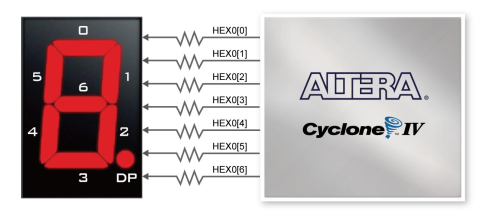
\includegraphics[width= 0.7\textwidth]{figures/chap2/hex.png}
                    \caption{\label{figure:hex} Connections between the 7-segment display HEX0 and Cyclone IV GX FPGA}
                \end{center}
            \end{figure}
    
    \section{LCD Display}
        The LCD module has built-in fonts and can be used to display text by sending appropriate
        commands to the display controller called HD44780. \autoref{tab:lcd} and \autoref{figure:lcd} shows the assignments of FPGA pins to the LCD.
        
        \newpage
            
            \begin{figure}[!ht]
                \begin{center}
                    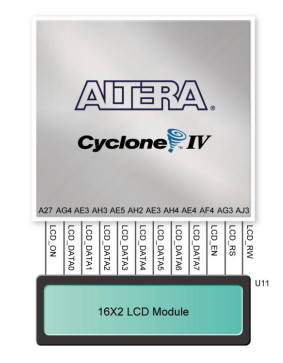
\includegraphics[width= 0.4\textwidth]{figures/chap2/lcd.png}
                    \caption{\label{figure:lcd} Connections between the LCD module and Cyclone IV GX FPGA}
                \end{center}
            \end{figure}
    
%%%%%%%%%%%%%%%%%%%%%%%%%%%%%%%%%%%%%%%%%%%%%%%%%%%%%%%%%%%%%%%%%%%%%%%%%%%%%%%%%%%%%%%%%%%%%%%%%%%%%%%%%

\chapter{Recording to the FPGA's Internal Memory} 

    In order for the Hardware described in VHDL to remain permanently in the FPGA, it is necessary to record it in the internal memory.
    
    \section {Step by step to record in internal memory}
    
        1. Open the .sof to .pof converter (programming object file)
        
        Path: In the File tab of Quartus II, open Convert Programming Files (Figure \ref{f1}).
        
            \begin{figure}[!ht]
                \begin{center}
                
                    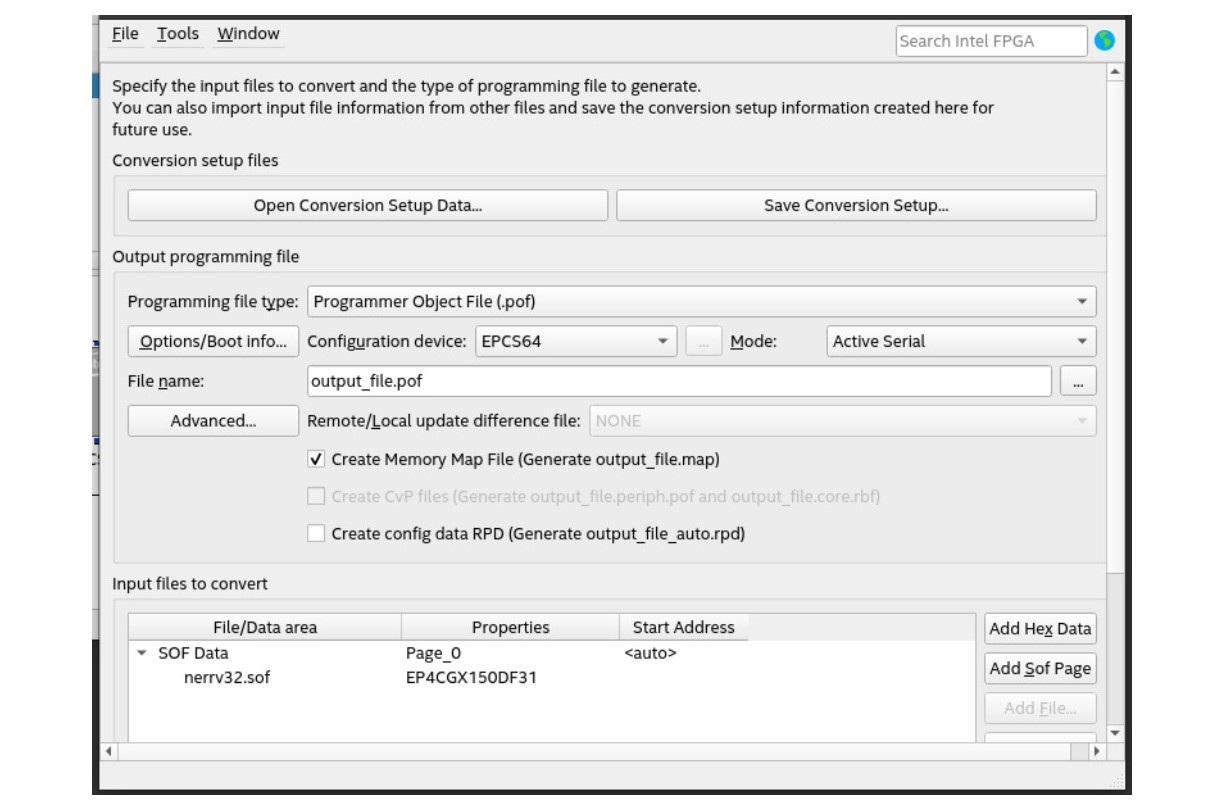
\includegraphics[width= 1\textwidth]{figures/chap2/fpga1.jpg}
                    \caption{\label{f1} Convert Programming Files Tool.}
                \end{center}
            \end{figure}
            
        2. On the FPGA switch to the recording mode (PROG) using the Programming Mode Switch shown in the Figure \ref{f2}.
        
            \begin{figure}[!ht]
                \begin{center}
                    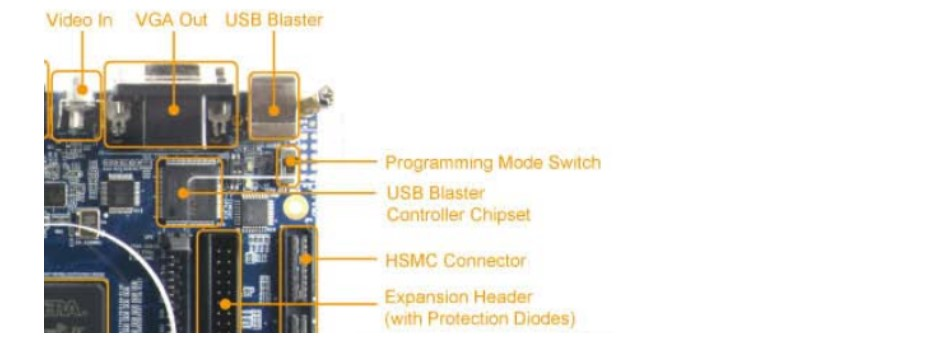
\includegraphics[width= 1\textwidth]{figures/chap2/fpga2.jpg}
                    \caption{\label{f2} Programming Switch Indication.}
                \end{center}
            \end{figure}
        
        3. Then open the Programmer via the path: Tools > Programmer.
            
            \begin{figure}[!ht]
                \begin{center}
                    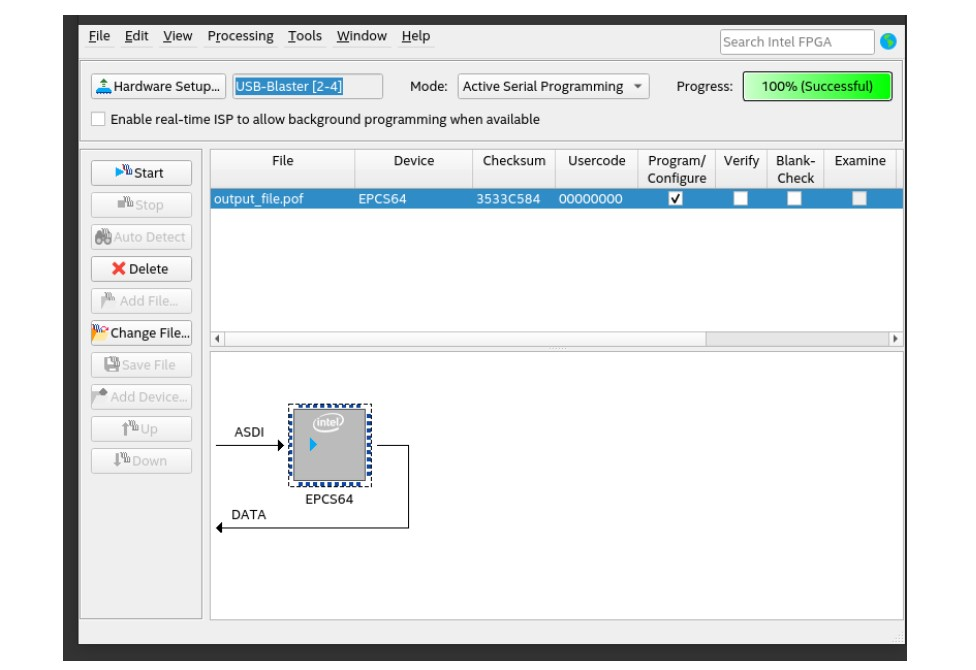
\includegraphics[width= 1\textwidth]{figures/chap2/fpga3.jpg}
                    \caption{\label{f3} Programmer Tool.}
                \end{center}
            \end{figure}
        
        4. Finally, Add Active Serial Programming, add the .pof file and click Start (Figure \ref{f3}). Before starting the FPGA, return the Programming Mode Switch to RUN mode.
        
%%%%%%%%%%%%%%%%%%%%%%%%%%%%%%%%%%%%%%%%%%%%%%%%%%%%%%%%%%%%%%%%%%%%%%%%%%%%%%%%%%%%%%%%%%%%%%%%%%%%%%%%%

\chapter{Compiling and executing your first program}
    https://www.overleaf.com/project/645bf9168256250a3c9f9d4f
    \section{Downloading and installing the toolchain}
    
        First, you should access \url{https://github.com/stnolting/riscv-gcc-prebuilt}, to download the most recent available toolchains (today, 21/05/2023, \textcolor{blue}{\textbf{rv32i-4.0.0}}). You should have now access to a .tar.gz file. Then, the next step, is to create the folder that the toolchain is going to be installed. You can open a terminal and type:
        
            \begin{lstlisting}[backgroundcolor = \color{lightgray}, language=bash]
                $ sudo mkdir /opt/riscv
            \end{lstlisting}
        
        Now, you need to navigate to the folder where the .tar.gz file was downloaded, like:
        
            \begin{lstlisting}[backgroundcolor = \color{lightgray}, language=bash]
                $ cd Downloads/
            \end{lstlisting}
            
        And then you have to extract the .tar.gz file to the folder previously created:
        
            \begin{lstlisting}[backgroundcolor = \color{lightgray}, language=bash]
                $ sudo tar -xzf <toolchain_version>.tar.gz -C /opt/riscv/
            \end{lstlisting}
            
        Finally, you should add the toolchain's bin folder to your system's PATH environment variable. You can open the .bashrc file:
        
            \begin{lstlisting}[backgroundcolor = \color{lightgray}, language=bash]
                $ sudo nano .bashrc
            \end{lstlisting}
            
        And then add the following line in the end of the .bashrc file:
        
            \begin{lstlisting}[backgroundcolor = \color{lightgray}, language=bash]
                export PATH="/opt/riscv/bin:$PATH"
            \end{lstlisting}
            
        To make sure everything works fine, navigate to the folder with the aplication examples and execute the following command:
        
            \begin{lstlisting}[backgroundcolor = \color{lightgray}, language=bash]
                $ make check
            \end{lstlisting}
        
        If everything is working fine you should se an "\textbf{OK}" appearing at the end, like in the \autoref{fig:successful_check}.
        
            \begin{figure}[!ht]
                \begin{center}
                    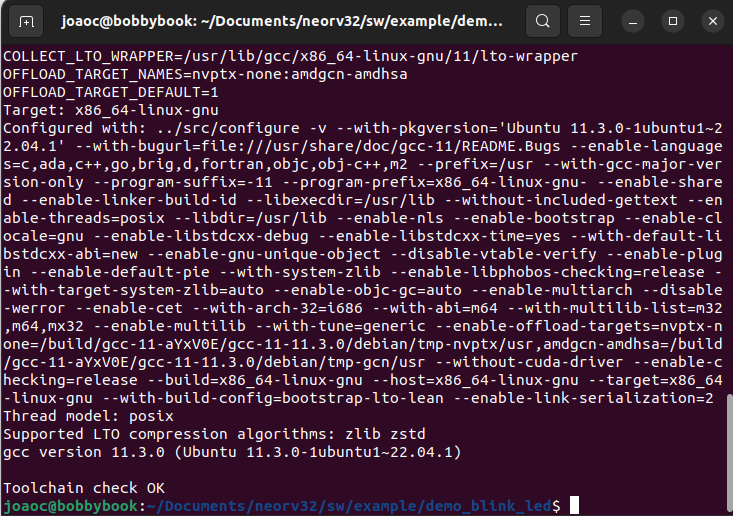
\includegraphics[width= 0.6\textwidth]{figures/successful_check.png}
                    \caption{Indication that the installation was successful.}
                    \label{fig:successful_check}
                \end{center}
            \end{figure}
    
        \subsection{Some important commands}
        
        Now that the toolchain was installed, you should know some commands to generate the .hex, .bin, .vdh, as well as other types of files. As you can see in \autoref{fig:toolchain_commands}, you could use \texttt{\hl{hex}} to generate the .hex file, which represents the machine language. You could use, for instance, the \texttt{\hl{image}} to generate the .vhd file, which is used to generate the \textit{neor32\_application\_image.vhd} that stores the main program that will run in the microprocessor. 
        
        
        \begin{figure}[!ht]
            \begin{center}
                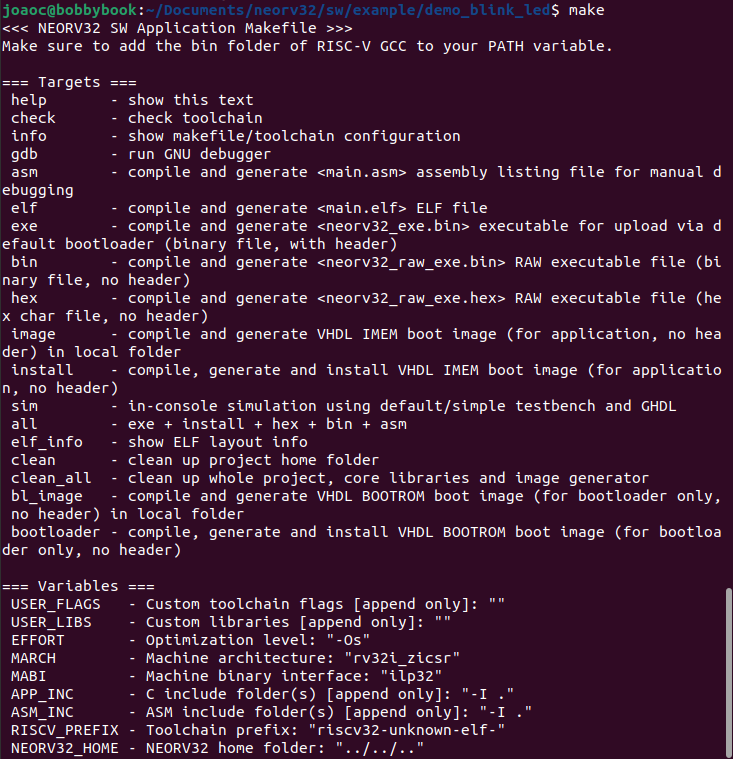
\includegraphics[width= 0.6\textwidth]{figures/toolchain_commands.png}
                \caption{Some useful commands to use.}
                \label{fig:toolchain_commands}
            \end{center}
        \end{figure}
        
    \section{Flash the program into FPGA Board using bootloader}
    
        In Linux, you should install a terminal emulator, like Minicom, Cutecom or similar:
        
            \begin{lstlisting}[backgroundcolor = \color{lightgray}, language=bash]
                $ sudo apt install cutecom
            \end{lstlisting}
        
        Then the software should be configured like in \autoref{fig:cutecom_configuration}.  With the FPGA previously programmed with the base of the NEORV32, you should see the status LED starts blinking and the bootloader intro screen appearing in your console, like:
        
            \begin{lstlisting}[backgroundcolor = \color{lightgray}, language=bash]
            
                << NEORV32 Bootloader >>
            
                BLDV: Mar  7 2023
                HWV:  0x01080107
                CID:  0x00000000
                CLK:  0x05f5e100
                MISA: 0x40901106
                XISA: 0xc0000fab
                SOC:  0xffff402f
                IMEM: 0x00008000 bytes @0x00000000
                DMEM: 0x00002000 bytes @0x80000000
            
                Autoboot in 8s. Press any key to abort.
            
            \end{lstlisting}
            
            \begin{figure}[!ht]
                \begin{center}
                    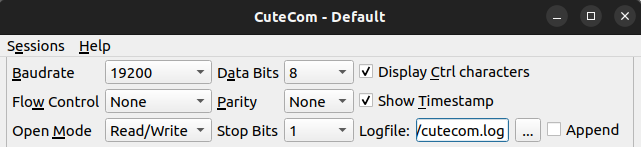
\includegraphics[width= 0.6\textwidth]{figures/cutecom_configuration.png}
                    \caption{Cutecom configuration.}
                    \label{fig:cutecom_configuration}
                \end{center}
            \end{figure}
            
        Now you can press any key to abort the automatic boot sequence and to start the actual bootloader user interface console. You then will have access to some commands, like:
        
            \begin{lstlisting}[backgroundcolor = \color{lightgray}, language=bash]
            
                Available CMDs:
                h: Help
                r: Restart
                u: Upload
                s: Store to flash
                l: Load from flash
                x: Boot from flash (XIP)
                e: Execute
                 
            \end{lstlisting}
        
        You can now upload the .bin file to execute it in the NEORV32. It will wait you to send the .bin file, so click on the \textit{send file} option to select the correct file. Finally, you can execute the program.
        
    \section{Flash the program into FPGA board directly}
        
        To generate an .vhd file for the IMEM that contains the actual application, run the \texttt{\hl{image}} inside the folder of your application. For instance, you could use any application from the NEORV32's examples folder, like neorv32-setup/sw/exmaple/demo\_blink\_led:
        
            \begin{lstlisting}[backgroundcolor = \color{lightgray}, language=bash]
                $ make clean_all image
            \end{lstlisting}
        
        This command will create the \textit{neorv32\_application\_image.vhd} file, that you can then add to the project's folder. If you are using Quartus II, you could replace the current application file or add it to the project if don't exists already.
    %
% examples.tex
%
% Copyright (C) 2023 UFSC.
%
% DOCUMENTATION-TEMPLATE
%
% This work is licensed under the Creative Commons Attribution-ShareAlike 4.0
% International License. To view a copy of this license,
% visit http://creativecommons.org/licenses/by-sa/4.0/.
%


\chapter{C Programming for Begginers}

    \section{Include Statements}
        These statements are used to introduce the contents of a separate file into your source file. This is a handy way to keep your code organized, and it also allows you to use library functionality, hardware-configuration routines, and register definitions provided by the manufacturer.
    
            \begin{lstlisting}[backgroundcolor = \color{lightgray}, language=c]
            //-------------------------------------------------------------
            // Includes
            //-------------------------------------------------------------
            #include // SFR declarations
            #include Project_DefsVarsFuncs.h
            #include InitDevice.h
            #include cslib_config.h
            #include cslib.h
            \end{lstlisting}

\section{Preprocessor Definitions}

    You can use a \#define statement to create a string that will be replaced by a number. Preprocessor definitions are not necessary, but in some situations they are extremely helpful because they allow you to easily modify a value that appears in various different portions of your program.
    
    
    For example, let’s say that you’re using the microcontroller’s ADC and that your code uses the ADC’s sample rate in several separate calculations. A preprocessor definition allows you to use an intuitive string (such as SAMPLE\_RATE) instead of the number itself in the calculation code, and if you’re experimenting with different sample rates, you only need to change the one numerical value in the preprocessor definition.
    
        \begin{lstlisting}[backgroundcolor = \color{lightgray}, language=c]
            #define SAMPLE_RATE 100000
        \end{lstlisting}
        
    You can change 100000 to any other number, and this new number will be used to replace all instances of the string SAMPLE\_RATE.

    Preprocessor definitions are also a great way to make code more readable. The following is a list of handy \#define statements.
     
        \begin{lstlisting}[backgroundcolor = \color{lightgray}, language=c]
        #define BIT7 0x80
        #define BIT6 0x40
        #define BIT5 0x20
        #define BIT4 0x10
        #define BIT3 0x08
        #define BIT2 0x04
        #define BIT1 0x02 
        #define BIT0 0x01
        
        #define HIGH 1
        #define LOW 0
        
        #define TRUE 1
        #define FALSE 0
        
        #define SET 1
        #define CLEARED 0
        
        #define LOWBYTE(v)   ((unsigned char) (v))
        #define HIGHBYTE(v)  ((unsigned char) (((unsigned int) (v)) >> 8))
        \end{lstlisting}

    Its important to understand that preprocessor definitions have no direct relationship to hardware. You’re just telling the preprocessor to replace one string of characters with another string of characters before the program is compiled.
    
        \subsection{Variables}
            Processors store data in registers and memory locations. There really is no such thing as a variable as far as the hardware is concerned. For the programmer, though, writing code is much easier when we can use intuitively named variables instead of memory addresses or register numbers.
            
            Compilers can manage the low-level details associated with variables without much input from the programmer, but if you want to optimize your use of variables you'll need to know something about the device’s memory configuration and the way in which it handles data of different bit widths.
            
            The following code excerpt gives an example of variable definition. This was written for the Keil Cx51 compiler, which reserves one byte of memory for an “unsigned char” definition, two bytes for an “unsigned int” definition, and four bytes for an “unsigned long” definition.
            
                 
                \begin{lstlisting}[backgroundcolor = \color{lightgray}, language=c]
                unsigned long Accumulated_Capacitance_Sensor1;
                unsigned long Accumulated_Capacitance_Sensor2;
                
                unsigned int Sensor1_Unpressed;
                unsigned int Sensor2_Unpressed;
                
                unsigned int Sensor1_Measurement;
                unsigned int Sensor2_Measurement;
                
                unsigned int AngularPosition;
                
                unsigned int TouchDuration;
                
                unsigned char CurrentDigit;
                unsigned int CharacterEntry;
                unsigned char DisplayDivider;
                \end{lstlisting}
                

        \subsection{Operators, Conditional Statements, and Loops} 
        
            The core of computational functionality consists of moving data, performing mathematical computations and logical operations with data, and making programmatic decisions based on the value of stored or generated data.
            
            Mathematical operations and bit manipulation are accomplished by means of operators. C has quite a few operators: equals (=), addition (+), subtraction (-), multiplication (*), division (/), bitwise AND (\&), bitwise OR (|), and so forth. The ``input'' to an operator statement are variables or constants, and the result is stored in a variable.
            
            Conditional statements allow you to perform or not perform an action based on whether a given condition is true or false. These statements use the words “if” and “else”; for example:
            
                \begin{lstlisting}[backgroundcolor = \color{lightgray}, language=c]
                if(Sensor1 < Sensor2 && Sensor1 < Sensor3)
                return SENSOR_1;
                
                else if(Sensor2 < Sensor1 && Sensor2 < Sensor3)
                return SENSOR_2;
                
                else if(Sensor3 < Sensor2 && Sensor3 < Sensor1)
                return SENSOR_3;
                
                else
                return 0;
                \end{lstlisting} 

            For loops and while loops provide a convenient means of repeatedly executing a block of code. These types of tasks arise very frequently in embedded applications. For loops are more oriented toward situations in which a block of code must be executed a specific number of times, and while loops are handy when the processor should continue repeating the same block of code until a condition changes from true to false. Here are examples of both types.

                \begin{lstlisting}[backgroundcolor = \color{lightgray}, language=c]
                for (n = 0; n < 16; n++)
                {
                Accumulated_Capacitance_Sensor1 += Measure_Capacitance(SENSOR_1);
                Delay_us(50);
                Accumulated_Capacitance_Sensor2 += Measure_Capacitance(SENSOR_2);
                Delay_us(50);
                }
                
                while(CONVERSION_DONE == FALSE);
                {
                LED_STATE = !LED_STATE;
                Delay_ms(100);
                }
                \end{lstlisting}
                
        \subsection{Functions} 

            Good C code is vastly superior to assembly code in terms of organization and readability, and this is due in large part to the use of functions.
            
            Functions are blocks of code that can be easily incorporated into other portions of code. Causing the processor to execute the instructions contained in the function is referred to as “calling” the function. A function can accept one or multiple inputs, and it can provide one output, called a return value.
            
            The use of functions does involve some overhead, so we have to be careful to not burden the processor with an excessive number of function calls, but in general the benefits of functions far outweigh the costs.
            
            Here is an example of a function that has three numerical inputs and uses these inputs to generate a true-or-false return value.
            
                \begin{lstlisting}[backgroundcolor = \color{lightgray}, language=c]
                bit Is_In_Range(int input, int LowerBound, int UpperBound)
                {
                if(input >= LowerBound && input <= UpperBound)
                  return TRUE;
                
                 else
                  return FALSE;
                }
                \end{lstlisting}
    
\chapter{Some examples}

    \section{GPIO}
    
    \section{7-segment Display}
    
    \section{LCD Display}
    
    \section{Interrupts}
    
    \section{Timer/Counter}
    
    \section{Serial UART}
    
    


    %
% references.tex
%
% Copyright (C) 2023 UFSC.
%
% DOCUMENTATION-TEMPLATE
%
% This work is licensed under the Creative Commons Attribution-ShareAlike 4.0
% International License. To view a copy of this license,
% visit http://creativecommons.org/licenses/by-sa/4.0/.
%

\bibliography{}

\addcontentsline{toc}{chapter}{References}

    %
% appendices.tex
%
% Copyright (C) 2023 UFSC.
%
% DOCUMENTATION-TEMPLATE
%
% This work is licensed under the Creative Commons Attribution-ShareAlike 4.0
% International License. To view a copy of this license,
% visit http://creativecommons.org/licenses/by-sa/4.0/.
%

\begin{appendices}

%
% fpga_output_gpio.tex
%
% Copyright (C) 2023 UFSC.
%
% DOCUMENTATION-TEMPLATE
%
% This work is licensed under the Creative Commons Attribution-ShareAlike 4.0
% International License. To view a copy of this license,
% visit http://creativecommons.org/licenses/by-sa/4.0/.
%


\chapter{FPGA Output GPIO Pinout}

\begin{table}[!htb]\scriptsize
    \centering
    \begin{tabular}{c c c c}
        \toprule[1.5pt]
        \textbf{Type} & \quad \quad \textbf{PIN} & \quad \quad \textbf{FPGA Pin} & \quad \quad \textbf{GPIO\_o}  \\
          
        \midrule
               & \quad \quad 0 & \quad \quad PIN\_AA25 & \quad \quad LEDG [0]\\
               & \quad \quad 1 & \quad \quad PIN\_AB25 & \quad \quad LEDG [1]\\
               & \quad \quad 2 & \quad \quad PIN\_F27  & \quad \quad LEDG [2]\\
        LEDG   & \quad \quad 3 & \quad \quad PIN\_F26  & \quad \quad LEDG [3]\\        
               & \quad \quad 4 & \quad \quad PIN\_W26  & \quad \quad LEDG [4]\\
               & \quad \quad 5 & \quad \quad PIN\_Y22  & \quad \quad LEDG [5]\\
               & \quad \quad 6 & \quad \quad PIN\_Y25  & \quad \quad LEDG [6]\\
               & \quad \quad 7 & \quad \quad PIN\_AA22 & \quad \quad LEDG [7]\\
            \bottomrule[1.5pt]
         
    \end{tabular}
    \caption{\label{tab:ledg} Green LEDs (output GPIO) pinout}
\end{table}


\begin{table}[!htb]\scriptsize
    \centering
    \begin{tabular}{c c c c}
        \toprule[1.5pt]
        \textbf{Type} & \quad \quad \textbf{PIN} & \quad \quad \textbf{FPGA Pin} & \quad \quad \textbf{GPIO\_o}  \\
        
               & \quad \quad 8  & \quad \quad PIN\_T23 & \quad \quad LEDR [0]\\
               & \quad \quad 9  & \quad \quad PIN\_T24 & \quad \quad LEDR [1]\\
               & \quad \quad 10 & \quad \quad PIN\_V27 & \quad \quad LEDR [2]\\
        LEDR   & \quad \quad 11 & \quad \quad PIN\_W25 & \quad \quad LEDR [3]\\        
               & \quad \quad 12 & \quad \quad PIN\_T21 & \quad \quad LEDR [4]\\
               & \quad \quad 13 & \quad \quad PIN\_T26 & \quad \quad LEDR [5]\\
               & \quad \quad 14 & \quad \quad PIN\_R25 & \quad \quad LEDR [6]\\
               & \quad \quad 15 & \quad \quad PIN\_T27 & \quad \quad LEDR [7]\\

    \end{tabular}
    \caption{\label{tab:ledr}Red LEDs (output GPIO) pinout}
\end{table}

\begin{table}[!htb]\scriptsize
    \centering 
    \begin{tabular}{c c c c}
        \toprule[1.5pt]
        \textbf{Type} & \quad \quad \textbf{PIN} & \quad \quad \textbf{FPGA Pin} & \quad \quad \textbf{GPIO\_o}  \\

               & \quad \quad 16 & \quad \quad PIN\_E15 & \quad \quad HEX0 [0]\\
               & \quad \quad 17 & \quad \quad PIN\_E12 & \quad \quad HEX0 [1]\\
               & \quad \quad 18 & \quad \quad PIN\_G11 & \quad \quad HEX0 [2]\\
        HEX0   & \quad \quad 19 & \quad \quad PIN\_F11 & \quad \quad HEX0 [3]\\        
               & \quad \quad 20 & \quad \quad PIN\_F16 & \quad \quad HEX0 [4]\\
               & \quad \quad 21 & \quad \quad PIN\_D16 & \quad \quad HEX0 [5]\\
               & \quad \quad 22 & \quad \quad PIN\_F14 & \quad \quad HEX0 [6]\\
        \hline
               & \quad \quad 23 & \quad \quad PIN\_G14 & \quad \quad HEX1 [0]\\
               & \quad \quad 24 & \quad \quad PIN\_B13 & \quad \quad HEX1 [1]\\
               & \quad \quad 25 & \quad \quad PIN\_G13 & \quad \quad HEX1 [2]\\
        HEX1   & \quad \quad 26 & \quad \quad PIN\_F12 & \quad \quad HEX1 [3]\\        
               & \quad \quad 27 & \quad \quad PIN\_G12 & \quad \quad HEX1 [4]\\
               & \quad \quad 28 & \quad \quad PIN\_J9  & \quad \quad HEX1 [5]\\
               & \quad \quad 29 & \quad \quad PIN\_G10 & \quad \quad HEX1 [6]\\    
        \hline
               & \quad \quad 30 & \quad \quad PIN\_G8   & \quad \quad HEX2 [0]\\
               & \quad \quad 31 & \quad \quad PIN\_G7   & \quad \quad HEX2 [1]\\
               & \quad \quad 32 & \quad \quad PIN\_F7   & \quad \quad HEX2 [2]\\
        HEX2   & \quad \quad 33 & \quad \quad PIN\_AG30 & \quad \quad HEX2 [3]\\        
               & \quad \quad 34 & \quad \quad PIN\_F6   & \quad \quad HEX2 [4]\\
               & \quad \quad 35 & \quad \quad PIN\_F4    & \quad \quad HEX2 [5]\\
               & \quad \quad 36 & \quad \quad PIN\_F10  & \quad \quad HEX2 [6]\\  
        \hline
               & \quad \quad 37 & \quad \quad PIN\_D10 & \quad \quad HEX3 [0]\\
               & \quad \quad 38 & \quad \quad PIN\_D7  & \quad \quad HEX3 [1]\\
               & \quad \quad 39 & \quad \quad PIN\_E6  & \quad \quad HEX3 [2]\\
        HEX3   & \quad \quad 40 & \quad \quad PIN\_E4  & \quad \quad HEX3 [3]\\        
               & \quad \quad 41 & \quad \quad PIN\_E3  & \quad \quad HEX3 [4]\\
               & \quad \quad 42 & \quad \quad PIN\_D5  & \quad \quad HEX3 [5]\\
               & \quad \quad 43 & \quad \quad PIN\_D4  & \quad \quad HEX3 [6]\\
               
        
    \end{tabular}
    \caption{\label{tab:hex}7-segments display (output GPIO) pinout}
\end{table}

\begin{table}[!htb]\scriptsize
    \centering
    \begin{tabular}{c c c c}
        \toprule[1.5pt]
        \textbf{Type} & \quad \quad \textbf{PIN} & \quad \quad \textbf{FPGA Pin} & \quad \quad \textbf{GPIO\_o}  \\
        
               & \quad \quad 44 & \quad \quad & \quad \quad\\
               & \quad \quad 45 & \quad \quad & \quad \quad\\
               & \quad \quad 46 & \quad \quad & \quad \quad\\
               & \quad \quad 47 & \quad \quad & \quad \quad\\        
               & \quad \quad 48 & \quad \quad & \quad \quad\\
               & \quad \quad 49 & \quad \quad & \quad \quad\\
               & \quad \quad 50 & \quad \quad & \quad \quad\\
               & \quad \quad 50 & \quad \quad & \quad \quad\\
        \bottomrule[1.5pt] 
    \end{tabular}
    \caption{\label{tab:empty}Available (output GPIO) pinout}
\end{table}

\begin{table}[!htb]\scriptsize
    \centering
    \begin{tabular}{c c c c}
        \toprule[1.5pt]
        \textbf{Type} & \quad \quad \textbf{PIN} & \quad \quad \textbf{FPGA Pin} & \quad \quad \textbf{GPIO\_o}  \\
        
               & \quad \quad 52 & \quad \quad PIN\_AG4 & \quad \quad DATA [0]\\
               & \quad \quad 53 & \quad \quad PIN\_AF3 & \quad \quad DATA [1]\\
               & \quad \quad 54 & \quad \quad PIN\_AH3 & \quad \quad DATA [2]\\
               & \quad \quad 55 & \quad \quad PIN\_AE5 & \quad \quad DATA [3]\\        
               & \quad \quad 56 & \quad \quad PIN\_AH2 & \quad \quad DATA [4]\\
               & \quad \quad 57 & \quad \quad PIN\_AE3 & \quad \quad DATA [5]\\
        LCD    & \quad \quad 58 & \quad \quad PIN\_AH4 & \quad \quad DATA [6]\\  
               & \quad \quad 59 & \quad \quad PIN\_AE4 & \quad \quad DATA [7]\\ 
               & \quad \quad 60 & \quad \quad PIN\_AF4 & \quad \quad EN\\
               & \quad \quad 61 & \quad \quad PIN\_AJ3 & \quad \quad RW\\
               & \quad \quad 59 & \quad \quad PIN\_AG3 & \quad \quad RS\\
               & \quad \quad 59 & \quad \quad PIN\_AF27 & \quad \quad ON\\
        \bottomrule[1.5pt]
    \end{tabular}
    \caption{\label{tab:lcd}LCD display (output GPIO) pinout}
\end{table}

\end{appendices}




\end{document}
